\documentclass[manuscript]{acmart}
\usepackage{graphicx} 
\usepackage[numbers]{natbib}

%% Removing the ACM Reference Format text block
\setcopyright{none}
\settopmatter{printacmref=false}
\renewcommand\footnotetextcopyrightpermission[1]{}
\pagestyle{plain}

%%

\title{A Novel Interactive System to Combat Household Food Waste}
\author{Group 10}
\date{October 2025}


\begin{document}


\maketitle

% --- TABLE OF CONTENTS ---
% Exclude the Table of Contents (Not in word Coubt)
\tableofcontents
\newpage

% --- REPORT BODY ---

% ----------------------------------------------------------------------
% SECTION 1: INTRODUCTION AND BACKGROUND
% ----------------------------------------------------------------------
\newpage
\section{Introduction and background}
% This section should be ~2-3 pages
% Describe the problem domain (sustainability, specifically food waste)
% Detail the social and technical challenges
% Showcase our motivation and what makes the project novel
\subsection{Problem Domain.}
We have chosen the domain of sustainability for our project. Sustainability is a an umbrella term for projects and practices concerned with meeting present needs without compromising the ability of  future generations to meet theirs. It involves solving environmental, economic, and social issues, focusing on how resources can be managed more responsibly to reduce waste and environmental impact. Our project targets domestic food waste, one of the most persistent and overlooked contributors to unsustainable living. Tackling this issue isn't a simple single solution approach but requires changes in technology and behaviour. Particularly regarding encouraging individuals to make more efficient use of resources; lower their carbon footprint; and develop lasting habits that promote sustainable consumption for the long-term.  
\par

\subsection{Technical challenges within the domain.}
\begin{itemize}
    \item It may be difficult to get the information on a product easily - the barcode may not always contain the expiry date or may be damaged and unreadable (NOTE FOR EDITOR: barcodes don't contain any information useful for us yet, only 2D next gen barcodes, likely going to have to scan the expiry date)
    \item 
\end{itemize}
\par

\subsection{Societal challenges within the domain.}
Society as a whole faces a significant challenge in it's goal to reduce emissions to combat climate change. According to the Food and Agriculture Organization of the United Nations (FAO), agricultural industries emitted approximately 16.2 billion tonnes of CO2 globally in 2022, accounting for 29.7 percent of total greenhouse gas emissions \footnote{Food and Agriculture Organization of the United Nations (FAO) (2024) Greenhouse gas emissions from agrifood systems: Global, regional and country trends, 2000–2022. Rome: FAO. Available at: https://openknowledge.fao.org/handle/20.500.14283/cd3167en
 (Accessed: 22 October 2025).}. Additionally, the UK Waste and Resources Action Programme (WRAP) estimates 10.7 million tonnes of food were wasted in the United Kingdom in 2021 \footnote{House of Commons Library (2024) Food waste in the UK (Research Briefing CBP-7552). London: House of Commons Library. Available at: https://commonslibrary.parliament.uk/research-briefings/cbp-7552
 (Accessed: 22 October 2025).}. Much of the food wasted in the UK results from everyday consumer habits, including forgetting about perishable items and not planning meals effectively around expiry dates. This is a widespread issue arising from the fact that keeping a note of expiry dates is both tedious and time-consuming. Additionally, many students struggle to plan a meal last minute using an ingredient which they have just discovered is near its expiry date or purchase too much food resulting in products expiring before it can be used. 

Currently, there are few widely adopted solutions to this problem, with existing expiry-tracking applications, like Beep, often being inaccessible due to high subscription fees. Amid an ongoing cost-of-living crisis in the UK, many students face tight budgets and limited disposable income. Reducing food waste not only lowers grocery expenses but also contributes to a more sustainable and environmentally responsible lifestyle.  To help prevent food waste students need to be able to keep a track of their foods' expiration dates with reminders as it's approaching without taking too much of their time; to be able to plan meals last minute and in advance with their perishable ingredients so nothing is wasted; make smarter decisions when purchasing food.
\par

\subsection{Motivation for the project.}
As busy students, it is difficult to keep track of food expiration dates and to plan meals accordingly. This leads to a significant amount of food being wasted every week, which is not only economically costly but also environmentally irresponsible. We feel that as sustainability-focused young people it is our responsibility to develop a solution that reduces food waste and the associated emissions. Too often, short-shelf-life items are forgotten at the back of the fridge, only to be thrown away days later. By developing a smart expiry-date tracking system, we aim to help students save money, reduce waste, and make more sustainable consumption choices. We are motivated to solve this problem as it affects us personally, and many of us would make use of the solution ourselves. 
\par

\subsection{Novel aspects of the project. }
While other solutions tackling this problem do exist, they have issues that we intend to solve. Namely:
\begin{itemize}
    \item Paid subscription models and low ratings for key features in existing solutions, examples being Plan to Eat\footnote{https://www.plantoeat.com} and Remy\footnote{https://www.remyapp.io} among others 
    \item Disjoint features from several apps that could be unified under one solution
    \item User Experience (\textbf{ELABORATE})
\end{itemize}
\label{sec:introduction}
% About 2-3 pages


% ----------------------------------------------------------------------
% SECTION 2: STAKEHOLDERS AND THEIR GOALS
% ----------------------------------------------------------------------
\newpage
\section{Stakeholders and their goals}
% This section should be ~ 1-2 pages
% Describe primary, secondary, and other stakeholders
% Detail their context, needs, and desired goals/experiences
\subsection{Primary Stakeholders}
    \indent\indent \textit{Students} - Students, particularly those who have recently become independent, are the target audience for our app as this demographic contributes disproportionately to food waste in the UK. Entering into a new environment with increased responsibilities results in many students becoming neglectful of less present problems such as the food expiring in their fridge. The WRAP UK Household Food Management Survey 2024\cite{waringPleaseUseThis} supports this assertion, attributing increased household food waste to traits highly prevalent among students\cite{gamboa-delgadoFactorsAssociatedFood2024, landryBarriersCollegeStudent2024} including competency and living circumstances – 49\% of “those who judge themselves weaker at judging and buying the right amount [of food]” and 31\% of “those who agree to feeling under time pressure” were categorized as high food wasters, clearly exceeding the population mean of 27\%. Through surveying students from several universities\cite{STUDENT SURVEY, FRESHER SURVEY} we uncovered that the majority of students “sometimes” disposed of food items due to them being out of date, with this being especially pervasive among first year students. The primary reasons cited for this wastage were “I forgot it was there” and “I was unable to use all of the ingredient”. From this response we have decided to tailor our app to include notifications to remind students about food expiry dates as well as a meal recommendation feature for leftovers, with the desired outcome being to reduce the responsibility for students to check their food and plan their meals so that the amount of expired food items students dispose of weekly decreases.\\
    \par
    \textit{Developers} – As developers we are the technical specialists responsible for designing, building and maintaining the app. Our role is to ensure that the app is both efficient and meets the users’ needs, particularly with regards to features such as date code scanning, expiry date notifications and meal recommendations for leftovers. We are therefore directly affected by the app in the forms of workload, technical challenges and app maintenance. Consequently, our goal is to produce a reliable, effective, secure app that achieves our goal of reducing the amount of unnecessary food waste produced by students and other demographics. \\
    \par
    \textit{Other Primary Stakeholders include:} Parents and Other Potential App Users
\subsection{Secondary Stakeholders}
    \indent\indent \textit{Supermarkets} – Supermarkets will be indirectly affected by our app since it is intended to empower consumers to better manage their food at home, reducing household waste that originates from supermarket purchases. This strengthens the supermarket’s sustainability profile and enhances their reputation for environmental responsibility. Our app would therefore aim to align with the major objectives of supermarkets\cite{WRAPSRETAILSURVEY} – being to strengthen their drive for environmental sustainability, enhance customer loyalty, and gain insights into post-purchase food management – while balancing potential impacts on sales volumes. Furthermore, future app iterations could potentially see users receiving expiry dates directly from the supermarket checkouts, deepening collaboration between the app and supermarket and so reinforcing customer loyalty towards both the app and supermarket.\\
    \par
    \textit{Local Councils} – In the long-term local councils will be indirectly affected by our app and so are considered secondary stakeholders. By reducing food waste among individual students, parents and other users, communities will consequently see a reduction in food waste. As of 2022 local authorities in the UK have been mandated to reduce food waste by prioritising household waste prevention through public behaviour change\cite{peacockLocalAuthorityCollected}, while also ensuring weekly separate food waste collections that divert unavoidable waste from landfill to recycling or energy recovery. Moreover, in March 2024 the UK Government announced a “new £295 million for councils to introduce weekly food waste collection”\cite{NewPS295mCouncils}, money local councils could reallocate to address other local issues (such as increased local public transport\cite{HowLocalTransport2024}) if they faced less pressure to reduce food waste. The desired outcome of our app towards local councils would be to alleviate the financial and political pressure created by high food waste among communities, allowing them to reduce money allocated to food waste and instead focus it towards other more pressing issues.\\
    \par
    \textit{Other Secondary Stakeholders Include:} Housemates, the Taxpayer
\subsection{Tertiary Stakeholders}
	\indent\indent \textit{Our Tertiary Stakeholders Include:} Environmental NGO’s and Sustainability Organisations (e.g. WRAP), Policy Makers\\
    \\

\begin{figure}[h!]
\centering
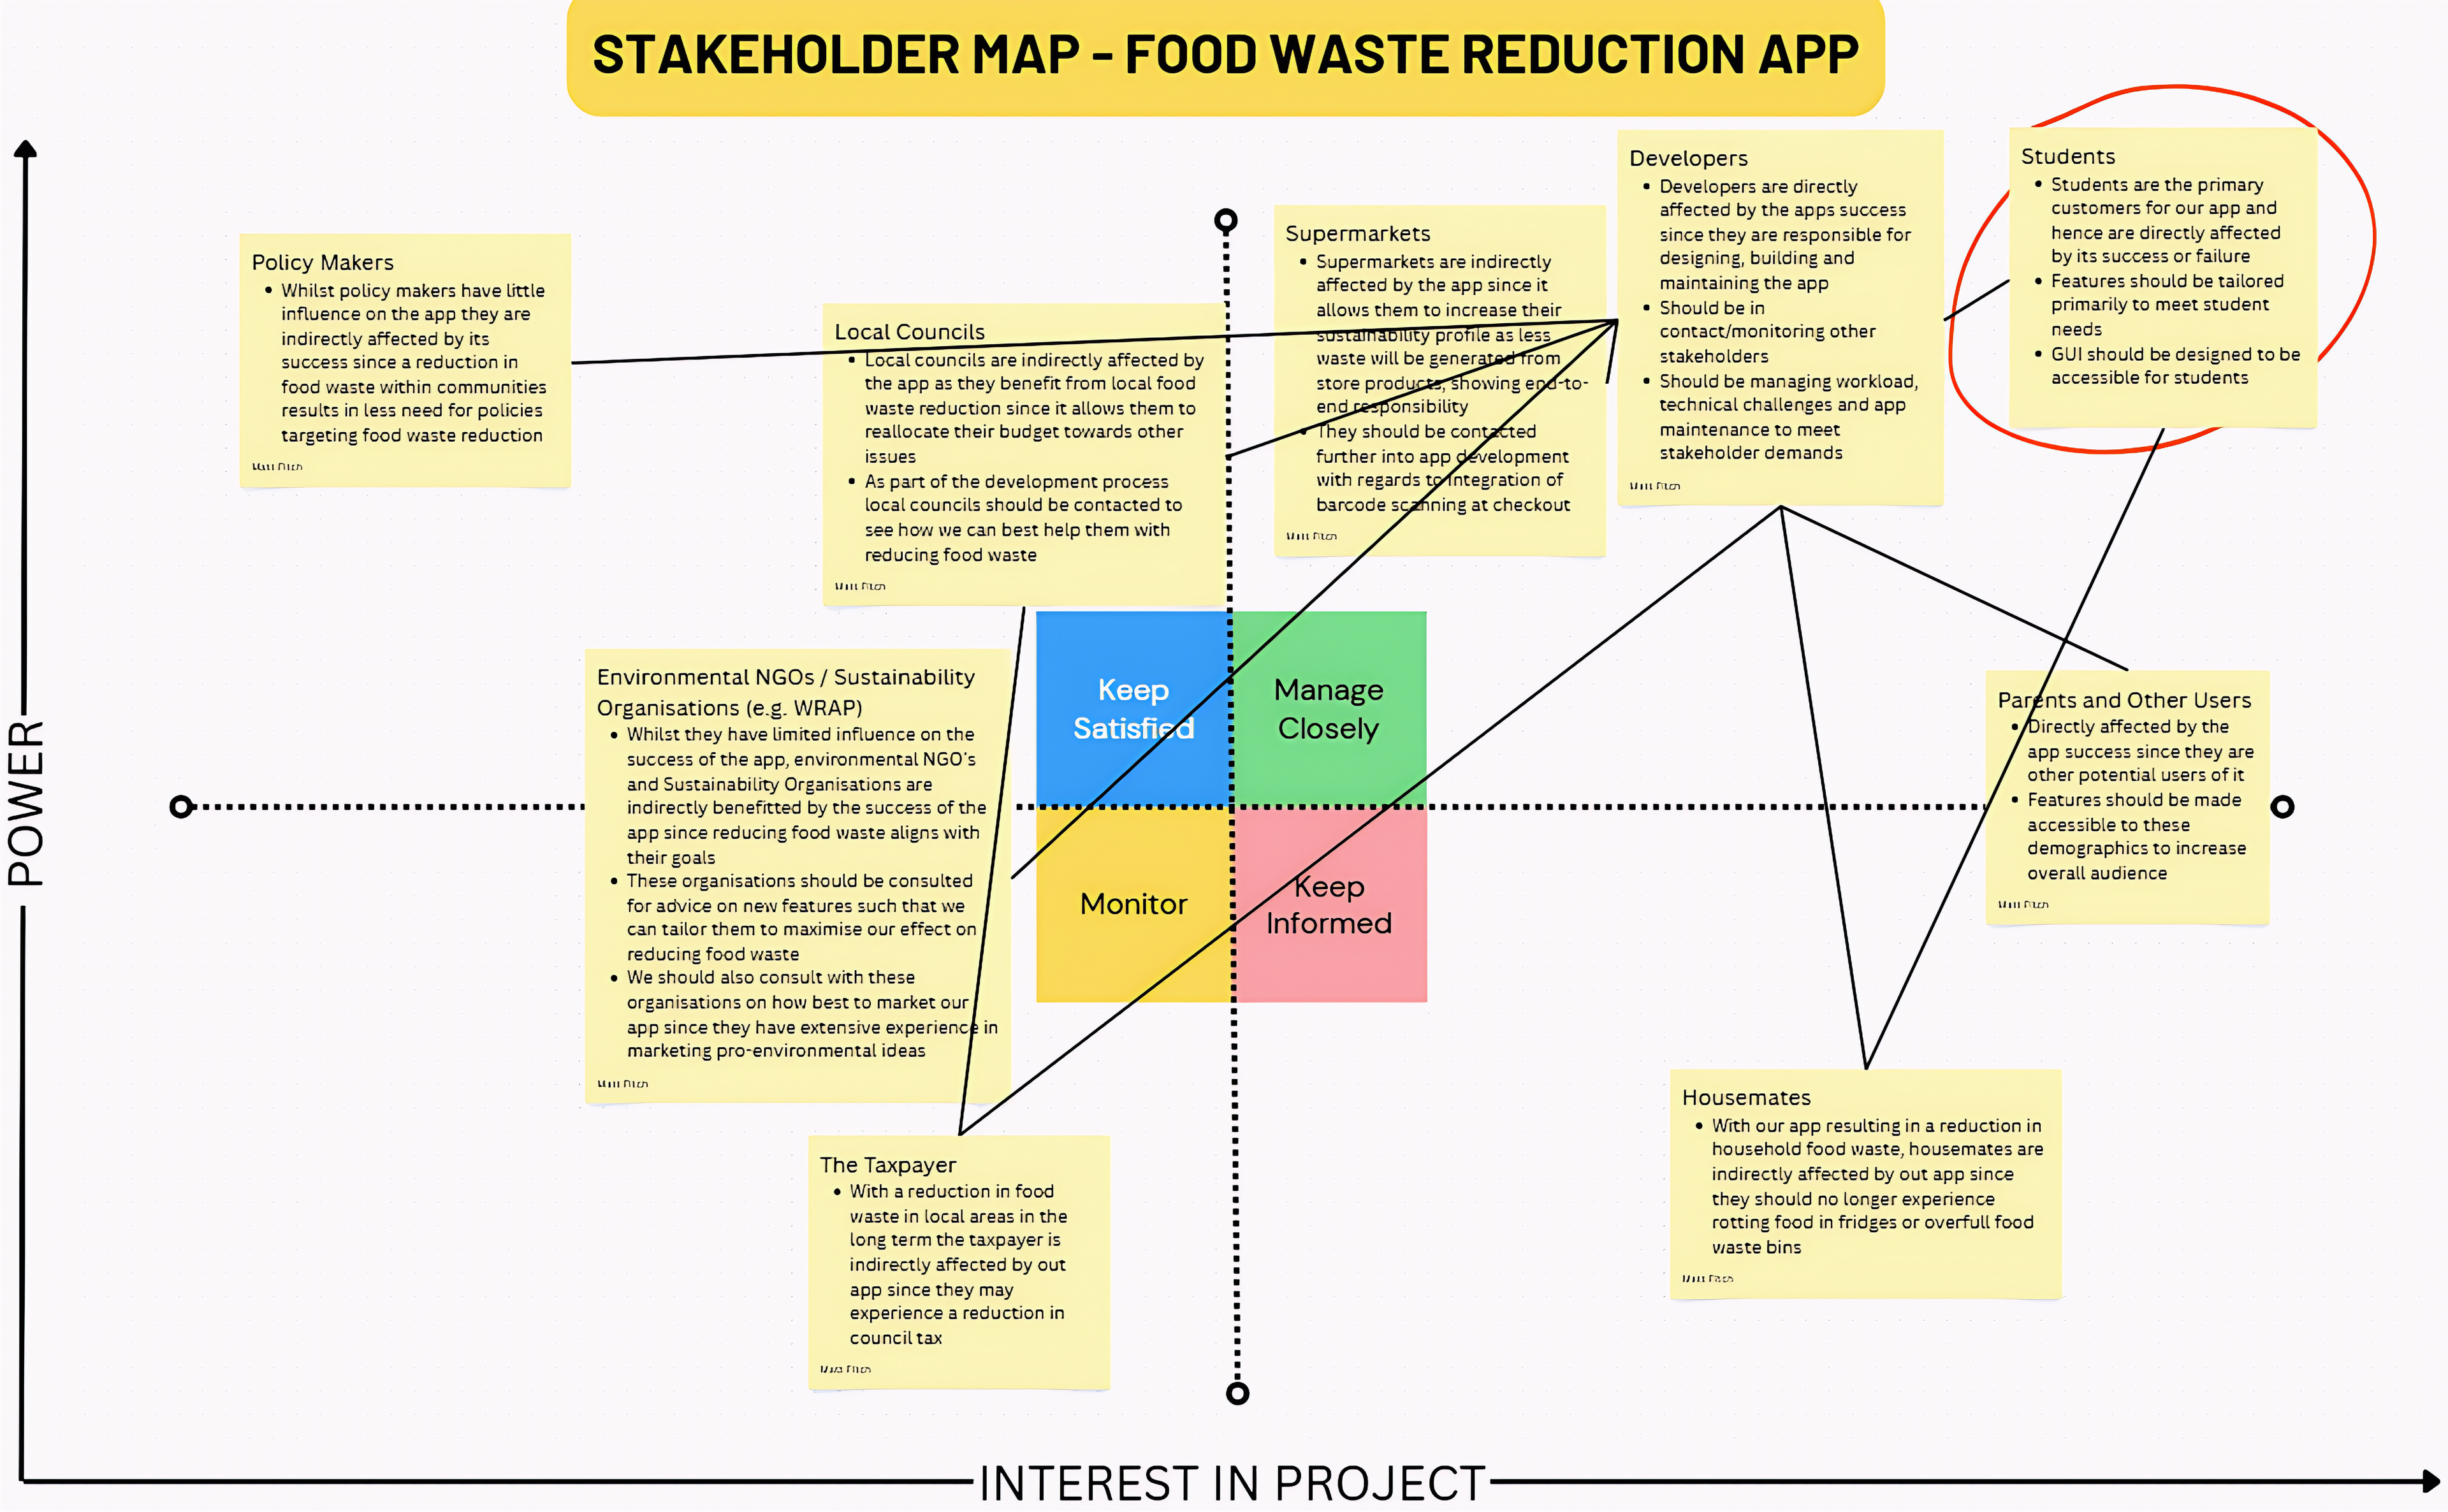
\includegraphics[width=1\linewidth]{Stakeholder Map - FWRA_imgupscaler.ai_General_4K.jpg}
\caption{\label{fig: Stakeholder Map}Stakeholder Map}
\end{figure}





\label{sec:stakeholders}
% About 1-2 pages



% ----------------------------------------------------------------------
% SECTION 3: PROJECT GOALS AND THE PROPOSED SYSTEM
% ----------------------------------------------------------------------
\newpage 
\section{Project goals and the proposed system}
% This section should be ~2-3 pages
% Clearly state the problem you are solving and your project's goal
% Introduce the system and its user benefits in implementation free terms
% Describe our customer measures of success
% Include a competitor analysis
Little Intro...
\subsubsection{Stakeholder/Customer Problem Statement and Project Goal}
\subsubsection{The Proposed Novel Interactive System:}
\subsubsection{User Benefitis in Implementation-Free Terms}
\subsubsection{Supporting Stakeholder Goals}
\subsubsection{Stakeholder-Centric Measures of Success}
\subsubsection{Potential NegativeImpacts Of The Proposed System}
3.6.1 Legal Implications
3.6.2 Ethical Implications
3.6.3 Professional Implications


\label{sec:project-goals}
% About 2-3 pages


% ----------------------------------------------------------------------
% SECTION 4: PROJECT MANAGEMENT AND THE TEAM
% ----------------------------------------------------------------------
\newpage

\section{Project management and the team}
% This section should be ~2-3 pages
% Describe our development process (Agile/Scrum)
% Justify our choice of tools, languages, libraries
% Detail your plants for testing, evaluation, and work distribution
\subsubsection{Development Process}
Since we are not developing safety critical software, we can use a more agile approach
to developing software, which ensures that we are meeting stakeholder requirements and prioritizing
the most important features. This also allows us to present more concrete software for feedback.
\par 

\subsubsection{Tools}
We will be using Github to track our changes, allowing us to work simultaneously, 
track issues, and keep track of who is working on what. 
Github's CI/CD will also be used to detect any errors added from commited code.
\par
For scheduling we could use a kanban board to track what tasks need completing and seeing
progress for current tasks. Alternatively we could use Github's issue section to manage
the activities needing completion. This comes at the drawback of being harder to track progress
for.
\subsubsection{Language / Libraries}

For developing Android applications, we can choose from Python using Kivy or Java using the Android SDK.
Python's Kivy module looks to have good documentation
\footnote{https://kivy.org/doc/stable/api-kivy.html}.
For Java, there are two possible choices for documentation:
\begin{enumerate}
  \item Using the official Android site
    \footnote{https://developer.android.com/reference/android/package-summary}
  \item Devdoc provides a simpler alternative
    \footnote{https://devdoc.net/android/Android-r15/reference/android/package-summary.html}
\end{enumerate}
\par
For libraries used, we will prioritize using popular well-known libraries, as they will have more
active security development reducing the likelihood of vulnerabilities. We will focus on using
open-source libraries which gives us the freedom to modify source code to adjust functionality to
better suit our needs, and to reduce cost, ensuring our product is available for our stakeholders.

\subsubsection{Testing}
We will be using Github's CI/CD tool to perform automatic regression testing for our software.
This ensures any added code doesn't break previous expectations.
Furthermore, for local development, we will integrate LSPs and formatting tools to quickly detect
simple bugs, as well as to ensure that the code has a consistent style to make navigating and understanding easier.
Beyond that, we will also ensure new features have appropriate tests added, as well as ensuring commits are
reviewed by at least one other person before merging feature to main.
\subsubsection{Evaluation}
\subsubsection{Work Distribution}
\subsubsection{Development Process}
Since we are not developing safety critical software, we can use a more agile approach
to developing software, which ensures that we are meeting stakeholder requirements and prioritizing
the most important features. This also allows us to present more concrete software for feedback.
\par 

\subsubsection{Tools}
We will be using Github to track our changes, allowing us to work simultaneously, 
track issues, and keep track of who is working on what. 
Github's CI/CD will also be used to detect any errors added from commited code.
\par
For scheduling we could use a ka\subsubsection{Development Process}
Since we are not developing safety critical software, we can use a more agile approach
to developing software, which ensures that we are meeting stakeholder requirements and prioritizing
the most important features. This also allows us to present more concrete software for feedback.
\par 
\subsubsection{Tools}
We will be using Github to track our changes, allowing us to work simultaneously, 
track issues, and keep track of who is working on what. 
Github's CI/CD will also be used to detect any errors added from commited code.
\par
For scheduling we could use a kanban board to track what tasks need completing and seeing
progress for current tasks. Alternatively we could use Github's issue section to manage
the activities needing completion. This comes at the drawback of being harder to track progress
for.
\subsubsection{Language / Libraries}
For developing Android applications, we can choose from Python using Kivy or Java using the Android SDK.
Python's Kivy module looks to have good documentation
\footnote{https://kivy.org/doc/stable/api-kivy.html}.
For Java, there are two possible choices for documentation:
\begin{enumerate}
  \item Using the official Android site
    \footnote{https://developer.android.com/reference/android/package-summary}
  \item Devdoc provides a simpler alternative
    \footnote{https://devdoc.net/android/Android-r15/reference/android/package-summary.html}
\end{enumerate}
\par
For libraries used, we will prioritize using popular well-known libraries, as they will have more
active security development reducing the likelihood of vulnerabilities. We will focus on using
open-source libraries which gives us the freedom to modify source code to adjust functionality to
better suit our needs, and to reduce cost, ensuring our product is available for our stakeholders.
\subsubsection{Testing}
We will be using Github's CI/CD tool to perform automatic regression testing for our software.
This ensures any added code doesn't break previous expectations.
Furthermore, for local development, we will integrate LSPs and formatting tools to quickly detect
simple bugs, as well as to ensure that the code has a consistent style to make navigating and understanding easier.
Beyond that, we will also ensure new features have appropriate tests added, as well as ensuring commits are
reviewed by at least one other person before merging feature to main.
\subsubsection{Evaluation}
\subsubsection{Work Distribution}
nban board to track what tasks need completing and seeing
progress for current tasks. Alternatively we could use Github's issue section to manage
the activities needing completion. This comes at the drawback of being harder to track progress
for.
\subsubsection{Language / Libraries}

For developing Android applications, we can choose from Python using Kivy or Java using the Android SDK.
Python's Kivy module looks to have good documentation
\footnote{https://kivy.org/doc/stable/api-kivy.html}.
For Java, there are two possible choices for documentation:
\begin{enumerate}
  \item Using the official Android site
    \footnote{https://developer.android.com/reference/android/package-summary}
  \item Devdoc provides a simpler alternative
    \footnote{https://devdoc.net/android/Android-r15/reference/android/package-summary.html}
\end{enumerate}
\par
For libraries used, we will prioritize using popular well-known libraries, as they will have more
active security development reducing the likelihood of vulnerabilities. We will focus on using
open-source libraries which gives us the freedom to modify source code to adjust functionality to
better suit our needs, and to reduce cost, ensuring our product is available for our stakeholders.

\subsubsection{Testing}
We will be using Github's CI/CD tool to perform automatic regression testing for our software.
This ensures any added code doesn't break previous expectations.
Furthermore, for local development, we will integrate LSPs and formatting tools to quickly detect
simple bugs, as well as to ensure that the code has a consistent style to make navigating and understanding easier.
Beyond that, we will also ensure new features have appropriate tests added, as well as ensuring commits are
reviewed by at least one other person before merging feature to main.
\subsubsection{Evaluation}
\subsubsection{Work Distribution}

\label{sec:project-management}


% ----------------------------------------------------------------------
% SECTION 5: CONSTRAINTS AND RISKS
% ----------------------------------------------------------------------
\newpage
\section{Constraints and Risks}
% This section should be ~1 page.
% Describe any constraints (technical, legal, ethical, etc.)
% Identify potential risks and your plans to mitigate them
% A table is  effective here for risk assessment
These are the factors that will limit our design, implementation, and deployment:
\begin{enumerate}

\item Legal and Regulatory Constraints

\begin{itemize}

\item Data Privacy (GDPR): \\
Constraints around collecting and storing user data (e.g., location, purchasing habits) and the need for transparent Consent Mechanisms.

\item Food Labelling Compliance: \\
Need to ensure the app's information presentation doesn't conflict with or misrepresent Official Food Labeling Regulations (e.g., the legal definition of "Best Before" vs. "Use By"). The app must be clearly an informational tool, not a definitive legal authority.

\item Platform/App Store Policies: \\
Adherence to strict rules set by Google Play and Apple App Store (e.g., security, payment systems, content).

\end{itemize}

\item Ethical and Social Constraints

\item Professional and Policy Constraints

\end{enumerate}

\par

There are potential problems that could negatively affect the project's success, the following actions are planned to prevent or reduce their impact:

\begin{center}
\begin{tabular}{| p{2cm} | p{5cm} | p{7cm} |}
    \hline
    \textbf{Risk Category} & \textbf{Potential Risk} & \textbf{Mitigation Plan} \\
    \hline
    Technical & Inaccurate Scanning and Data Entry (e.g., misreading an expiry date, linking to the wrong product). & A clear training protocol and double-checking process for data entry specialists. \\
    \hline
    User Adoption & Lack of User Engagement (users stop scanning items after the initial novelty wears off). & Focus on a Seamless User Experience (minimal steps to log an item), Gamification elements (e.g., tracking food waste reduction score), and Push Notifications (gentle reminders for items nearing expiration). \\
    \hline
    Data/Security & Data Breach or Misuse of Personal Data (e.g., purchasing history is compromised). & Ensure Encryption in Transit and at Rest for all personal data. Use anonymisation or aggregation techniques where possible. Conduct regular Security Audits and adhere to OWASP Top 10 guidelines. \\
    \hline
    Resource/Scope & Project features expand beyond initial capacity, leading to delays. & Maintain a strict Minimum Viable Product (MVP) definition. Use a formal change request process for all new feature suggestions. Prioritize features based on their Direct Impact on Food Waste Reduction. \\
    \hline
    External & Major Manufacturer Changes (e.g., a dominant supermarket changes its QR code format or packaging). & Develop a Modular Scanning System that can be rapidly updated to accommodate changes in labeling formats. Establish an Ongoing Data Maintenance schedule. \\
    \hline
\end{tabular}
\end{center}

% ----------------------------------------------------------------------
% SECTION 6: REFERENCES
% ----------------------------------------------------------------------
\newpage
\bibliographystyle{bathx}
\bibliography{bibliography}


% ----------------------------------------------------------------------
% SECTION 7: APPENDICES
% ----------------------------------------------------------------------
\newpage
\appendix
\section{Stakeholder Survey Data}
\subsection{Survey Questions}


\subsection{Responses}
Responses to the "First Year" Survey:

Responses to the "Second Year and Above" Survey:

Responses to the "Parents" Survey:

Notes:
Data from the "First Year" Survey and the "Second Year and Above" Survey was collected from University students attending the universities of Bath, Cambridge, Oxford, LSE and Durham.
Data from the "Parents" Survey was collected from parents in the Surrey area
\subsection{Raw Data}
The full raw survey data for all three forms is provided as supplementary material in the files:
\begin{itemize}
  \item Appendix\_Raw-Data\_StakeholderSurveyFirstYear.xlsx
  \item Appendix\_Raw-Data\_StakeholderSurveySecondYearandAbove.xlsx
  \item Appendix\_Raw-Data\_StakeholderSurveyParents.xlsx
\end{itemize}

\newpage
\section{Additional Data - REMOVE IF NOT NEEDED}
\subsection{Meeting Minutes}
\subsection{Meeting Notes}
More content in a second appendix.
\end{document}